\documentclass[12pt]{article}
\usepackage{xcolor}
\usepackage[top=2cm, bottom=2cm, left=2cm, right=2cm, headsep=2mm, foot=4mm]{geometry}
\usepackage{amsmath,amsthm,amsfonts,amssymb,amscd}
\usepackage{enumerate}
\usepackage{parskip}
\usepackage{mathtools}
\usepackage{mathrsfs}
\usepackage{mdframed}
\usepackage{verbatimbox}
\usepackage{graphicx}
\graphicspath{ {./img/} }

\title{Homework 1 - AMATH 583}
\author{Warren Paris-Moe}
\date{April 2023}

\begin{document}
\maketitle

\section{Level 1 BLAS (Basic Linear Algebra Subprograms)}
\begin{mdframed}
    Given the following specification, write a C++ function that computes $y \leftarrow \alpha x + y$, 
    where $x,y \in \mathbb{R^n}, \alpha \in \mathbb{R}$. Write a C++ code that calls the function
    and measures the performance for $n = 2$ to $n = 1024$. Let each $n$ be measured ntrial times and plot the
    average performance for each case versus $n$, $\text{ntrial} \geq 3$ (performance is FLOPs don’t forget).
    You may initialize your problem with any non-zero values you desire (random numbers are good). 
    The correctness of your function will be tested against a test system with known result, so please test 
    prior to submission. Check for and flag incorrect cases. Submit C++ function file, main source file, and 
    performance plot.
    \begin{verbnobox}[\small]
    void daxpy (double a, const std::vector<double> &x, std::vector<double> &y);
    \end{verbnobox}
\end{mdframed}

\begin{figure}[h!]
    \centering
    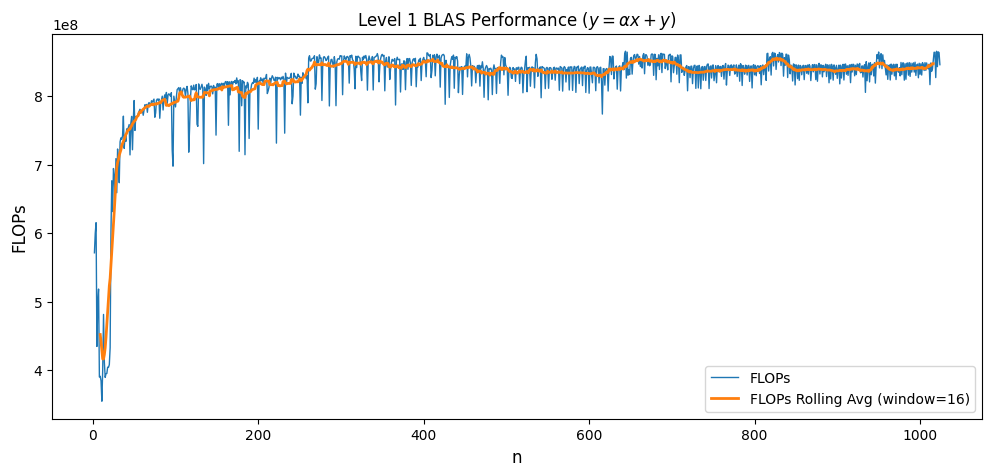
\includegraphics[scale=0.65]{img/q1-plot.png}
    \caption{Level 1 BLAS Performance for $n \in [2,1024]$, \textit{ntrial=1000}.}
    \label{fig:level1blas}
\end{figure}

\section{Level 1 BLAS Loop Unrolled}
\begin{mdframed}
    Given the following specification, write a C++ function that computes $y \leftarrow \alpha x + y$, 
    where $x,y \in \mathbb{R^n}, \alpha \in \mathbb{R}$. Your function should unroll the loop at least 
    to depth 4, and accept a block size parameter. Write a C++ code that calls the function
    and measures the performance for $n=2048$ and study the block sizes 1,2,4,8,16,32,64. 
    Measure \textit{ntrial} times for each block size and plot the average performance for each case 
    versus $n$, $ntrial \geq 3$. You may initialize your problem with any non-zero values you desire 
    (random numbers are good). The correctness of your function will be tested against a test system 
    with known result, so please test prior to submission. Check for and flag incorrect cases. 
    Submit C++ function file, main source file, and performance plot.
    % wrap the text in verbnobox to prevent line breaks
    \begin{verbnobox}[\small]
        void daxpy_unroll (double a, const std::vector<double> &x, 
        std::vector<double> &y, int blocksize);
    \end{verbnobox}
\end{mdframed}


\end{document}
